\documentclass{article}
\usepackage[utf8]{inputenc}
\usepackage{amsmath}
\usepackage{amssymb}
\usepackage{graphicx}

\begin{document}

\section*{Block-wise LU decomposition}
We are given a block-partitioned matrix $A \in \mathbb{R}^{n+1, n+1}$ that looks like
\begin{equation*}
    \mathbf{A} = 
    \begin{bmatrix}
    \mathbf{R} & \mathbf{v} \\
    \mathbf{u}^{\mathsf{T}} & 0
    \end{bmatrix}
\end{equation*}
where $\mathbf{u}, \mathbf{v}\in \mathbb{R}^{n}$ and $\mathbf{R}\in\mathbb{R}^{n,n}$ is \textbf{upper triangular} and regular.
\subsection*{2-3.a} 
We are tasked with refreshing our knowledge on the LU-decomposition of a matrix. 

\begin{figure}[!hbt]
    \centering
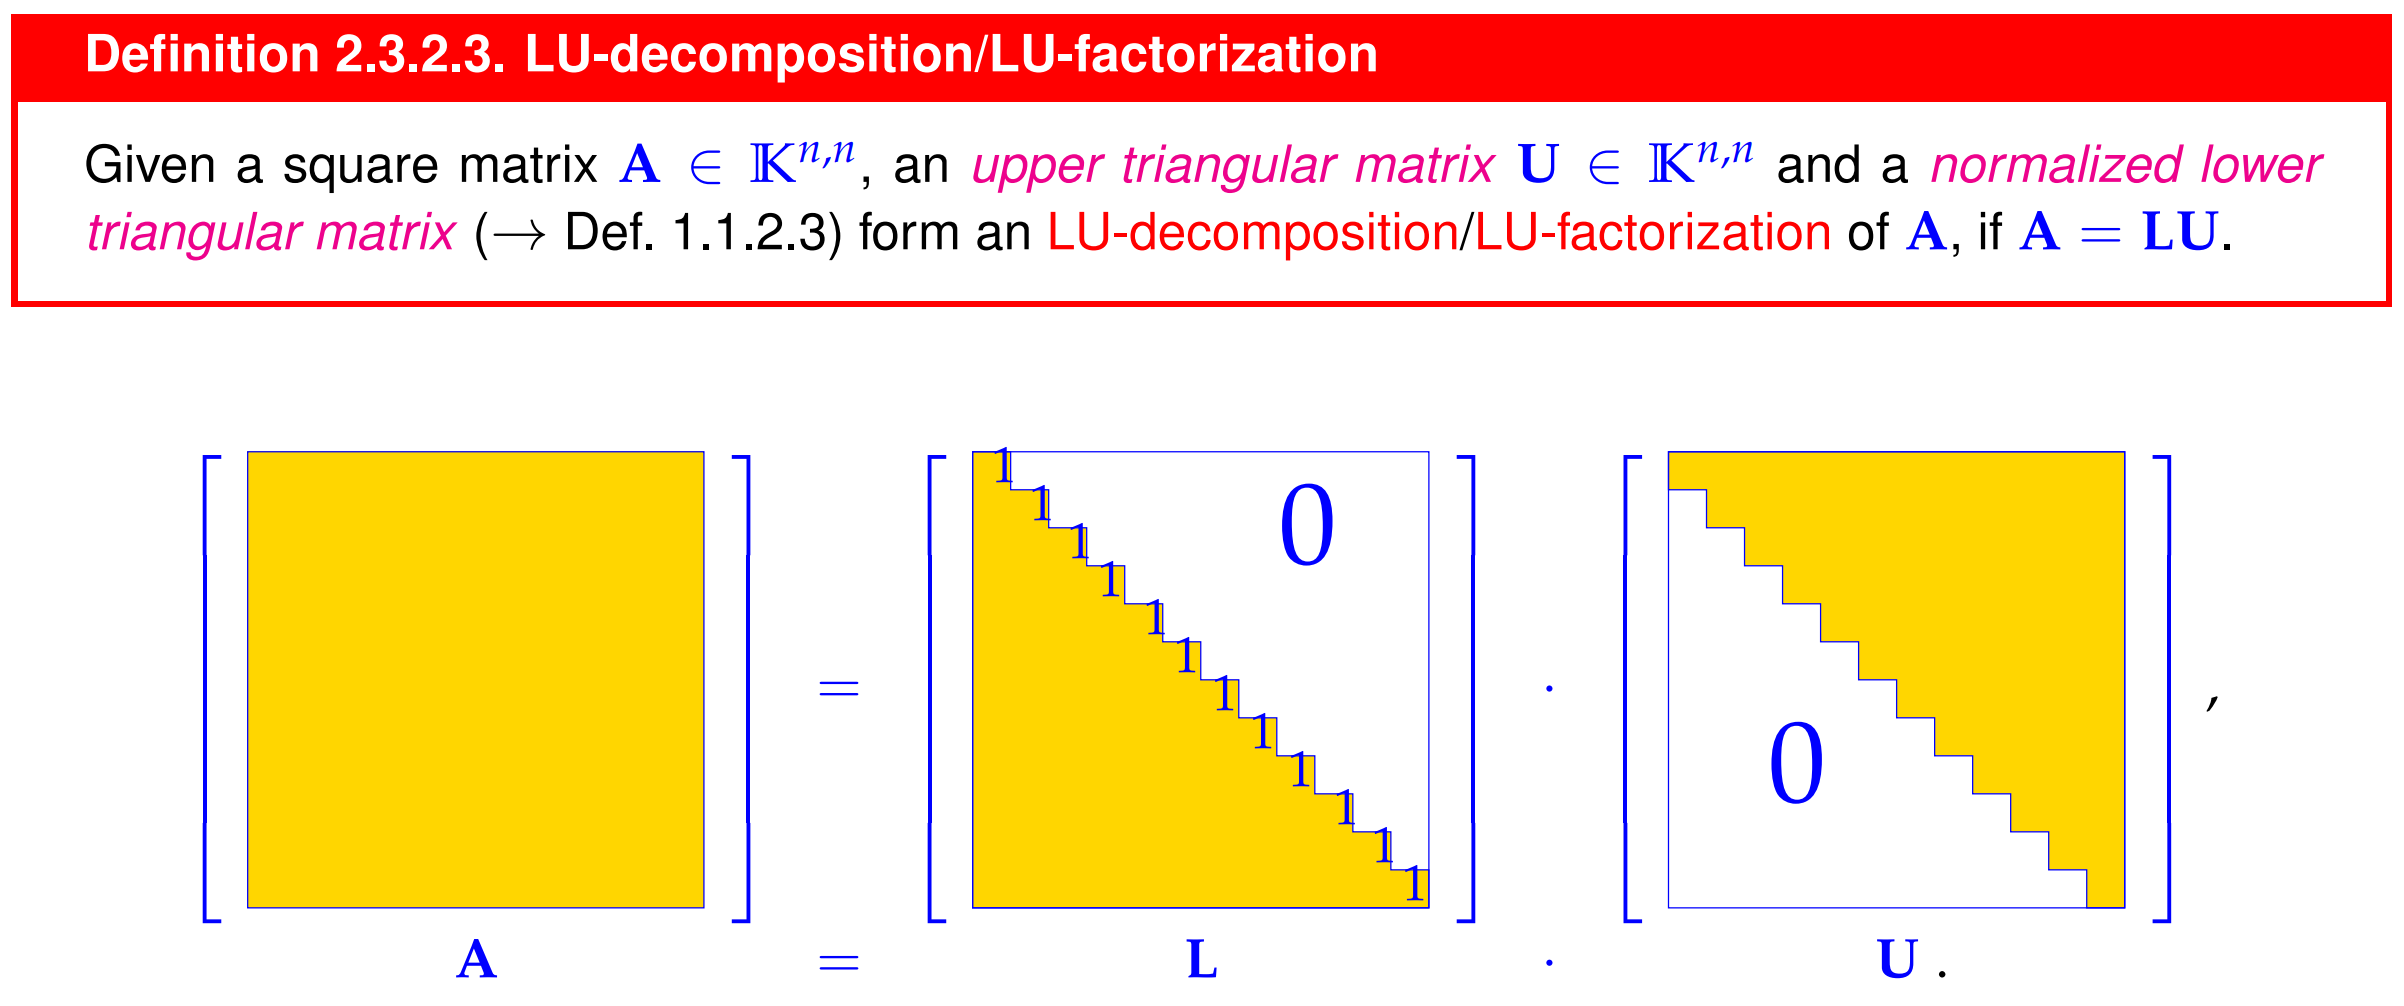
\includegraphics[width=1.0\linewidth]{LUFactorization.png}
\end{figure}

\noindent We have seen that the LU-factorization can be done using forward Gaussian elimination, which then give us an asymptotic complexity of $\mathcal{O}\left(n^{2}\right)$.
\subsection*{2-3.b}
We are now tasked with finding the LU-decomposition of the matrix $\mathbf{A}$ from above. We have seen in remark 2.3.2.19 how one can do block LU-factorization. The general form for a matrix $A$ composed into four blocks like
\begin{equation*}
    \mathbf{A} = \begin{bmatrix}
        \mathbf{A}_{11} & \mathbf{A}_{12} \\
        \mathbf{A}_{21} & \mathbf{A}_{22}
    \end{bmatrix}
\end{equation*}
we can do the following block LU-factorization 
\begin{equation*}
  \begin{bmatrix}
        \mathbf{A}_{11} & \mathbf{A}_{12} \\
        \mathbf{A}_{21} & \mathbf{A}_{22}
    \end{bmatrix}  =
    \begin{bmatrix}
        \mathbf{I} & \mathbf{O} \\
        \mathbf{A}_{21}\mathbf{A}_{11}^{-1} & \mathbf{I}
    \end{bmatrix}
    \begin{bmatrix}
        \mathbf{A}_{11} & \mathbf{A}_{12} \\
        \mathbf{O} & \mathbf{S}
    \end{bmatrix}
\end{equation*}
Where we have that $\mathbf{S}$ is the \textbf{Schur complement} given by
\begin{equation*}
    \mathbf{S} := \mathbf{A}_{22} - \mathbf{A}_{21}\mathbf{A}_{11}^{-1}\mathbf{A}_{12}
\end{equation*}
Hence the only block that must be invertible (regular) is $\mathbf{A}_{11}$.

\pagebreak

\noindent Let us now apply this to the given matrix $\mathbf{A}$
\begin{equation*}
    \mathbf{A} = 
    \begin{bmatrix}
    \mathbf{R} & \mathbf{v} \\
    \mathbf{u}^{\mathsf{T}} & 0
    \end{bmatrix} = 
    \begin{bmatrix}
        \mathbf{I} & 0 \\
        \mathbf{u}^{\mathsf{T}}\mathbf{R}^{-1} & 1
    \end{bmatrix}
    \begin{bmatrix}
        \mathbf{R} & \mathbf{v} \\
        0 & \mathbf{S}
    \end{bmatrix}
\end{equation*}
The computation of the Schur complement gives us
\begin{equation*}
    \mathbf{S} = \mathbf{A}_{22} - \mathbf{A}_{21}\mathbf{A}_{11}^{-1}\mathbf{A}_{12} = 0 - \mathbf{u}^{\mathsf{T}}\mathbf{R}^{-1}\mathbf{v} =  - \mathbf{u}^{\mathsf{T}}\mathbf{R}^{-1}\mathbf{v}
\end{equation*}
This then gives us 
\begin{equation*}
     \mathbf{A} = \begin{bmatrix}
        \mathbf{I} & 0 \\
        \mathbf{u}^{\mathsf{T}}\mathbf{R}^{-1} & 1
    \end{bmatrix}
    \begin{bmatrix}
        \mathbf{R} & \mathbf{v} \\
        0 &  - \mathbf{u}^{\mathsf{T}}\mathbf{R}^{-1}\mathbf{v}
    \end{bmatrix}
\end{equation*}
\subsection*{2-3.c}
We are tasked with showing the following statement
\begin{equation*}
    \mathbf{A} \text{ is regular } \Longleftrightarrow - \mathbf{u}^{\mathsf{T}}\mathbf{R}^{-1}\mathbf{v} \neq 0
\end{equation*}
We show both sides of the equivalence. 
\paragraph{"$\Longrightarrow$":} Let us assume that $\mathbf{A}$ is regular. We now assume towards contradiction that $- \mathbf{u}^{\mathsf{T}}\mathbf{R}^{-1}\mathbf{v} = 0$, we then see that the LU-factorization is given by
\begin{equation*}
    \mathbf{A} = \begin{bmatrix}
        \mathbf{I} & 0 \\
        \mathbf{u}^{\mathsf{T}}\mathbf{R}^{-1} & 1
    \end{bmatrix}
    \begin{bmatrix}
        \mathbf{R} & \mathbf{v} \\
        0 & 0
    \end{bmatrix} = 
    \begin{bmatrix}
        \mathbf{R} & \mathbf{v} \\
    \mathbf{u}^{\mathsf{T}} & \mathbf{u}^{\mathsf{T}}\mathbf{R}^{-1}\mathbf{v}
    \end{bmatrix} = 
    \begin{bmatrix}
        \mathbf{R} & \mathbf{v} \\
        \mathbf{u}^{\mathsf{T}} & 0
    \end{bmatrix}
\end{equation*}
Where the last step follows because $ \mathbf{u}^{\mathsf{T}}\mathbf{R}^{-1}\mathbf{v} = -\mathbf{u}^{\mathsf{T}}\mathbf{R}^{-1}\mathbf{v} = 0$. We now use forward Gaussian elimination on the last matrix and get
\begin{align*}
    \begin{bmatrix}
        \mathbf{R} & \mathbf{v} \\
        \mathbf{u}^{\mathsf{T}} & 0
    \end{bmatrix} &\overset{-\mathbf{u}^{\mathsf{T}}\mathbf{R}^{-1}\text{ Row $1$}}{\longrightarrow}
    \begin{bmatrix}
        \mathbf{R} & \mathbf{v} \\
        \mathbf{u}^{\mathsf{T}}  -\mathbf{u}^{\mathsf{T}}\mathbf{R}^{-1}\mathbf{R} & 0 -\mathbf{u}^{\mathsf{T}}\mathbf{R}^{-1}\mathbf{v}
    \end{bmatrix} \\[2mm]
    &\hspace{20px}\longrightarrow
    \begin{bmatrix}
        \mathbf{R} & \mathbf{v} \\
        \mathbf{u}^{\mathsf{T}} -\mathbf{u}^{\mathsf{T}}\mathbf{I} &  -\mathbf{u}^{\mathsf{T}}\mathbf{R}^{-1}\mathbf{v}
    \end{bmatrix} \\[2mm]
     &\hspace{20px}\longrightarrow
    \begin{bmatrix}
        \mathbf{R} & \mathbf{v} \\
        \mathbf{u}^{\mathsf{T}} -\mathbf{u}^{\mathsf{T}} &  -\mathbf{u}^{\mathsf{T}}\mathbf{R}^{-1}\mathbf{v}
    \end{bmatrix} \\[2mm]
    &\hspace{20px}\longrightarrow
    \begin{bmatrix}
        \mathbf{R} & \mathbf{v} \\
        0 &  0
    \end{bmatrix}
\end{align*}
Where we used $- \mathbf{u}^{\mathsf{T}}\mathbf{R}^{-1}\mathbf{v} = 0$ in the last step. This matrix does not have full rank though, which contradicts our assumption that $\mathbf{A}$ is regular, thus we can follow that if $\mathbf{A}$ is regular we have $- \mathbf{u}^{\mathsf{T}}\mathbf{R}^{-1}\mathbf{v} \neq 0$, which concludes this direction of the proof.

\pagebreak

\paragraph{"$\Longleftarrow$":} Let us assume that we have $- \mathbf{u}^{\mathsf{T}}\mathbf{R}^{-1}\mathbf{v} \neq 0$ for the given LU-factorization of the matrix $\mathbf{A}$.
\begin{equation*}
     \mathbf{A} = \begin{bmatrix}
        \mathbf{I} & 0 \\
        \mathbf{u}^{\mathsf{T}}\mathbf{R}^{-1} & 1
    \end{bmatrix}
    \begin{bmatrix}
        \mathbf{R} & \mathbf{v} \\
        0 &  - \mathbf{u}^{\mathsf{T}}\mathbf{R}^{-1}\mathbf{v}
    \end{bmatrix}
\end{equation*}
We know that $\mathbf{R}$ is regular (we used this implicitly as well in the last proof), which we will use in this proof. Let us multiply these matrices.
\begin{align*}
    \begin{bmatrix}
        \mathbf{I} & 0 \\
        \mathbf{u}^{\mathsf{T}}\mathbf{R}^{-1} & 1
    \end{bmatrix}
    \begin{bmatrix}
        \mathbf{R} & \mathbf{v} \\
        0 &  - \mathbf{u}^{\mathsf{T}}\mathbf{R}^{-1}\mathbf{v}
    \end{bmatrix} &= 
    \begin{bmatrix}
        \mathbf{R} & \mathbf{v} \\
        \mathbf{u}^{\mathsf{T}}\mathbf{R}^{-1}\mathbf{R} &  \mathbf{u}^{\mathsf{T}}\mathbf{R}^{-1}\mathbf{v}- \mathbf{u}^{\mathsf{T}}\mathbf{R}^{-1}\mathbf{v}
    \end{bmatrix} \\[1mm]
    &=
    \begin{bmatrix}
        \mathbf{R} & \mathbf{v} \\
        \mathbf{u}^{\mathsf{T}}&  0
    \end{bmatrix}
\end{align*}
This result was known before but doing these steps helped me understand how exactly the decomposition works. We can now do forward Gaussian elimination on the matrix.

\begin{align*}
    \begin{bmatrix}
        \mathbf{R} & \mathbf{v} \\
        \mathbf{u}^{\mathsf{T}}&  0
    \end{bmatrix}
    \overset{-\mathbf{u}^{\mathsf{T}}\mathbf{R}^{-1}\text{ Row $1$}}{\longrightarrow}
    \begin{bmatrix}
        \mathbf{R} & \mathbf{v} \\
        \mathbf{u}^{\mathsf{T}} - \mathbf{u}^{\mathsf{T}}\mathbf{R}^{-1}\mathbf{R} & 
        - \mathbf{u}^{\mathsf{T}}\mathbf{R}^{-1}\mathbf{v}
    \end{bmatrix} &=  
    \begin{bmatrix}
        \mathbf{R} & \mathbf{v} \\
        \mathbf{u}^{\mathsf{T}} - \mathbf{u}^{\mathsf{T}}\mathbf{I} & 
        - \mathbf{u}^{\mathsf{T}}\mathbf{R}^{-1}\mathbf{v}
    \end{bmatrix} \\
    &= 
    \begin{bmatrix}
        \mathbf{R} & \mathbf{v} \\
        \mathbf{u}^{\mathsf{T}} - \mathbf{u}^{\mathsf{T}}& 
        - \mathbf{u}^{\mathsf{T}}\mathbf{R}^{-1}\mathbf{v}
    \end{bmatrix} \\
    &= 
    \begin{bmatrix}
        \mathbf{R} & \mathbf{v} \\
        \mathbf{0}^{\mathsf{T}}& 
        - \mathbf{u}^{\mathsf{T}}\mathbf{R}^{-1}\mathbf{v}
    \end{bmatrix}
\end{align*}
Because \mathbf{R} is regular the regularity of $\mathbf{A}$ depends entirely on the fact if $- \mathbf{u}^{\mathsf{T}}\mathbf{R}^{-1}\mathbf{v} \neq 0$ is true, which is the case by assumption, hence we get that $\mathbf{A}$ has full rank as none of the rows are eliminated to zero rows and the system is in upper triangular form. Hence it follows that \mathbf{A} is regular, which concludes this side of the proof as well and thus we have proven the statement from above.

\paragraph{Alternate proof:} One could use the fact that we have
\begin{equation*}
    \mathbf{A} \text{ is regular } \Longleftrightarrow \text{det}\left(\mathbf{A}\right) \neq 0
\end{equation*}
and use the equation
\begin{equation*}
    \text{det}\left(\mathbf{A}\mathbf{B}\right) = \text{det}\left(\mathbf{A}\right) \cdot \text{det}\left(\mathbf{B}\right)
\end{equation*}
to get the following result
\begin{equation*}
    \text{det}\left(\mathbf{A}\right) = 
    \text{det}\left(\mathbf{L}\right) \cdot 
    \text{det}\left(\mathbf{U}\right) = 
    \text{det}\left(\mathbf{L}\right) \cdot \text{det}\left(\mathbf{R}\right) \cdot \text{det}\left(-\mathbf{\mathbf{u}^{\mathsf{T}}\mathbf{R}^{-1}\mathbf{v}}\right) 
\end{equation*}
In the last step we used that we have the following result from linear algebra.
\begin{equation*}
    \text{det}
    \begin{bmatrix}
        \mathbf{A} & \mathbf{B} \\
        \mathbf{O} & \mathbf{D}
    \end{bmatrix} = \text{det }\mathbf{A}\text{ det }\mathbf{D}
    \quad \text{and} \quad 
    \text{det}
    \begin{bmatrix}
        \mathbf{A} & \mathbf{O} \\
        \mathbf{C} & \mathbf{D}
    \end{bmatrix} = \text{det }\mathbf{A}\text{ det }\mathbf{D}
\end{equation*}

\pagebreak

\noindent We know use that the determinant of triangular matrices is given by the product of the diagonal elements and hence $\text{det }\mathbf{L} = 1$, that $\mathbf{R}$ is regular and hence $\text{det }\mathbf{R} \neq 0$ and thus after rewriting the expression to ($\mathbf{u}^{\mathsf{T}}\mathbf{R}^{-1}\mathbf{v} \in \mathbb{R}$)
\begin{equation*}
    \text{det}\left(\mathbf{L}\right) \cdot \text{det}\left(\mathbf{R}\right) \cdot \text{det}\left(-\mathbf{\mathbf{u}^{\mathsf{T}}\mathbf{R}^{-1}\mathbf{v}}\right) = 
    \text{det}\left(\mathbf{L}\right) \cdot \text{det}\left(\mathbf{R}\right) \cdot \left(-\mathbf{\mathbf{u}^{\mathsf{T}}\mathbf{R}^{-1}\mathbf{v}}\right)
\end{equation*}
we can see that if $\mathbf{\mathbf{u}^{\mathsf{T}}\mathbf{R}^{-1}\mathbf{v}} = 0$, then so it the determinant of $\mathbf{A}$ and hence $\mathbf{A}$ is not regular, if $\mathbf{\mathbf{u}^{\mathsf{T}}\mathbf{R}^{-1}\mathbf{v}} \neq 0$ then also $\text{det }\mathbf{A} \neq 0$ and hence $\mathbf{A}$ is regular, which also proves the statement.
\subsection*{2-3.d}
We are now tasked with implementing a function that solves $\mathbf{A}\mathbf{x} = \mathbf{b}$ (and returns the result $\mathbf{x}$) for the $\mathbf{A}$ as described above, while using the block-LU-decomposition we derived in 2-3.b. Let us look at the block-LU-decomposition from 2-3.b.
\begin{equation*}
     \mathbf{A} = \begin{bmatrix}
        \mathbf{I} & 0 \\
        \mathbf{u}^{\mathsf{T}}\mathbf{R}^{-1} & 1
    \end{bmatrix}
    \begin{bmatrix}
        \mathbf{R} & \mathbf{v} \\
        0 &  - \mathbf{u}^{\mathsf{T}}\mathbf{R}^{-1}\mathbf{v}
    \end{bmatrix}
\end{equation*}
This gives us the system
\begin{equation*}
    \mathbf{A}\mathbf{x} = \begin{bmatrix}
        \mathbf{I} & 0 \\
        \mathbf{u}^{\mathsf{T}}\mathbf{R}^{-1} & 1
    \end{bmatrix}
    \begin{bmatrix}
        \mathbf{R} & \mathbf{v} \\
        0 &  - \mathbf{u}^{\mathsf{T}}\mathbf{R}^{-1}\mathbf{v}
    \end{bmatrix}\begin{bmatrix}
        \mathbf{x}_{1:n} \\ x_{n + 1}
    \end{bmatrix} = \begin{bmatrix}
        \mathbf{b}_{1:n} \\ b_{n + 1}
    \end{bmatrix}
\end{equation*}
We now first look at how we solve regular LSEs using LU-decomposition. Given $\mathbf{A} = \mathbf{L}\mathbf{U}$ we have
\begin{equation*}
    \mathbf{A}\mathbf{x} = \mathbf{L}\mathbf{U}\mathbf{x} = \mathbf{b}
\end{equation*}
We then first solve $\mathbf{L}\mathbf{y} = \mathbf{b}$ and then from this solve $\mathbf{U}\mathbf{x} = \mathbf{y}$. This can be done both of the times by solving an upper triangular systems of equations which can be done via backwards substitution. Let us look at the equations this gives us.
\begin{equation*}
    \mathbf{L}\mathbf{y} = \mathbf{b} \Longleftrightarrow \begin{bmatrix}
        \mathbf{I} & 0 \\
        \mathbf{u}^{\mathsf{T}}\mathbf{R}^{-1} & 1
    \end{bmatrix}\begin{bmatrix}
        \mathbf{y}_{1:n} \\y_{n + 1}
    \end{bmatrix} = 
    \begin{bmatrix}
        \mathbf{y}_{1:n} \\
        \mathbf{u}^{\mathsf{T}}\mathbf{R}^{-1}y_{1:n} + y_{n +1}
    \end{bmatrix}
    =
    \begin{bmatrix}
        \mathbf{b}_{1:n} \\b_{n +1}
    \end{bmatrix}
\end{equation*}
\begin{equation*}
    \mathbf{U}\mathbf{x} = \mathbf{y} \Longleftrightarrow \begin{bmatrix}
        \mathbf{R} & \mathbf{v} \\
        0 &  - \mathbf{u}^{\mathsf{T}}\mathbf{R}^{-1}\mathbf{v}
    \end{bmatrix}\begin{bmatrix}
        \mathbf{x}_{1:n} \\ x_{n +1}
    \end{bmatrix} = 
    \begin{bmatrix}
        \mathbf{y}_{1:n} \\
        y_{n +1}
    \end{bmatrix}
\end{equation*}
This system can be solved by backward substitution. The only thing left is computing $\mathbf{R}^{-1}$. Here we can again use the trick where for some dummy variable $\mathbf{\chi}$ we want to solve
\begin{equation*}
    \mathbf{R}\chi = \mathbf{v} \Longleftrightarrow  \chi = \mathbf{R}^{-1}\mathbf{v}
\end{equation*}
Because $\mathbf{R}$ is upper triangular this can also be solved by backwards substitution. We hence do the following steps.
\begin{enumerate}
    \item We compute $\mathbf{y}$ which requires only some computation because of the special structure of the matrix.
    \item We construct the matrix $\mathbf{U}$ by computing $\mathbf{R}^{-1}\mathbf{v}$ using backwards substitution.
    \item We solve the system $\mathbf{U}\mathbf{x} = \mathbf{y}$ using backwards substitution.
\end{enumerate}

\pagebreak

\noindent We first implement a function that does the backwards substitution. Let us for this consider a small upper triangular LSE as an example.
\begin{equation*}
    \begin{bmatrix}
        a_{11} & a_{12} & a_{13} \\
        0 & a_{21} & a_{22} \\
        0 & 0 & a_{33}
    \end{bmatrix}
    \begin{bmatrix}
        x_{1} \\
        x_{2} \\
        x_{3}
    \end{bmatrix}
    = \begin{bmatrix}
        b_{1} \\
        b_{2} \\
        b_{3}
    \end{bmatrix}
\end{equation*}
We do the following solving process
\begin{enumerate}
    \item Solve $a_{33}x_{3} = b_{3}$ which gives $x_{3} = \frac{b_{3}}{a_{33}}$
    \item Solve $a_{21}x_{2} + a_{22}x_{3}  = a_{21}x_{2} +\frac{b_{3}a_{22}}{a_{33}} = b_{2}$ This gives us $x_{2} = \frac{b_{2}}{a_{21}}-\frac{b_{3}a_{22}}{a_{33}a_{21}}$
    \item Repeat this step for the third equation.
\end{enumerate}
This translates into the following code.

\begin{figure}[!hbt]
    \centering
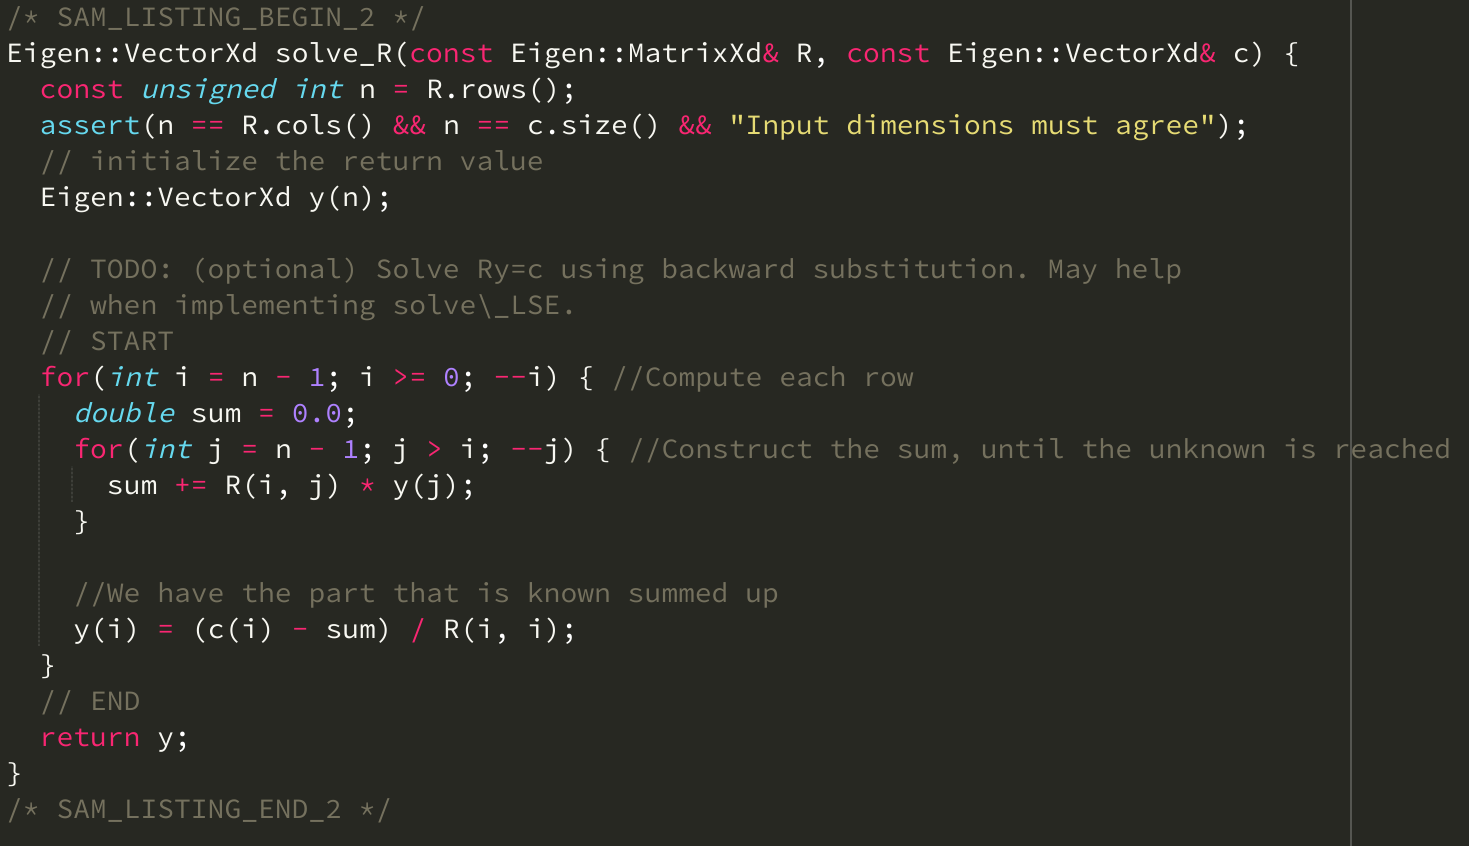
\includegraphics[width=0.7\linewidth]{2-3d.png}
\end{figure}

\noindent Now we follow the steps formulated above. We compute $\mathbf{R}^{-1}\mathbf{y}_{1:n-1}$ by again applying the trick as described above. This gives the following code.

\begin{figure}[!hbt]
    \centering
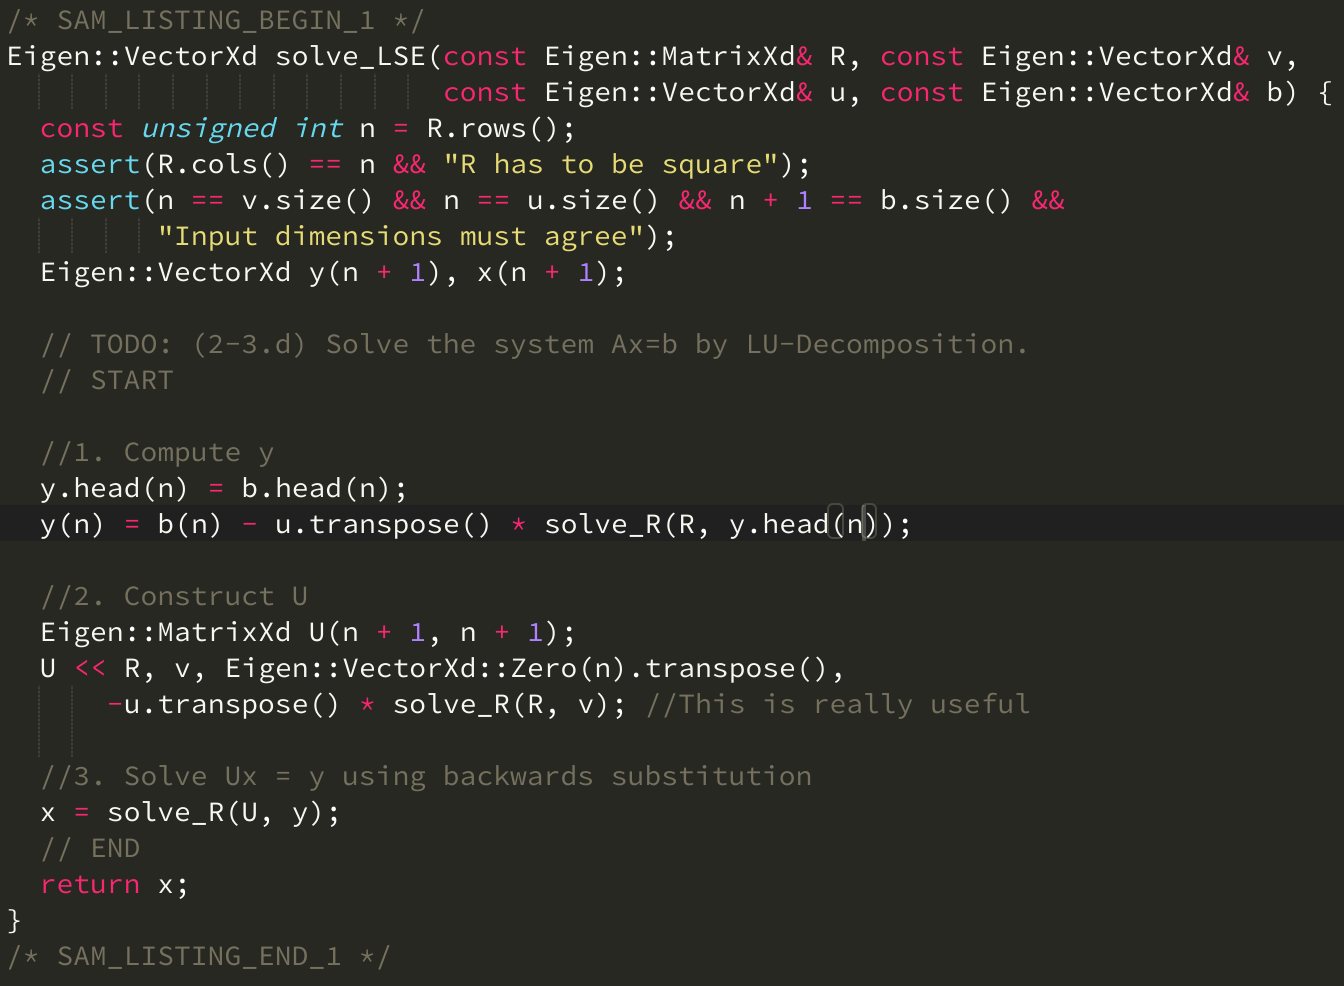
\includegraphics[width=0.7\linewidth]{2-3.d_part2.png}
\end{figure}

\end{document}
